\chapter{Specific Details on Training Activities and Report}
\label{chapter-3}

% Include:
% - Actual weekly activities performed
% - Specific tools used (replace examples)
% - Personal learning experiences
% - Project details with quantifiable outcomes

\section{Introduction}
\begin{itemize}
    \item Brief overview of the internship duration and host organization
    \item Key learning objectives and focus areas
    \item Technologies/tools used during training
    \item Summary of professional growth
\end{itemize}

\section{Weekly Duties and Activities}

\subsection{First Week: Overall Activity / Topic Name (e.g. Foundation)}
\begin{itemize}
    \item \textbf{Orientation:} Company introduction and team onboarding
    \item \textbf{Key Concepts Learned:}
    \begin{itemize}
        \item Software testing fundamentals
        \item SDLC (Stages as mentioned Fig.~\ref{fig:sdlc}), and STLC methodologies
        \item Testing types (manual/automation)
    \end{itemize}
\end{itemize}

\textcolor{red}{(You have to refer and describe every Figure you mentioned in your report like above)}

\begin{figure}[H]
    \centering
    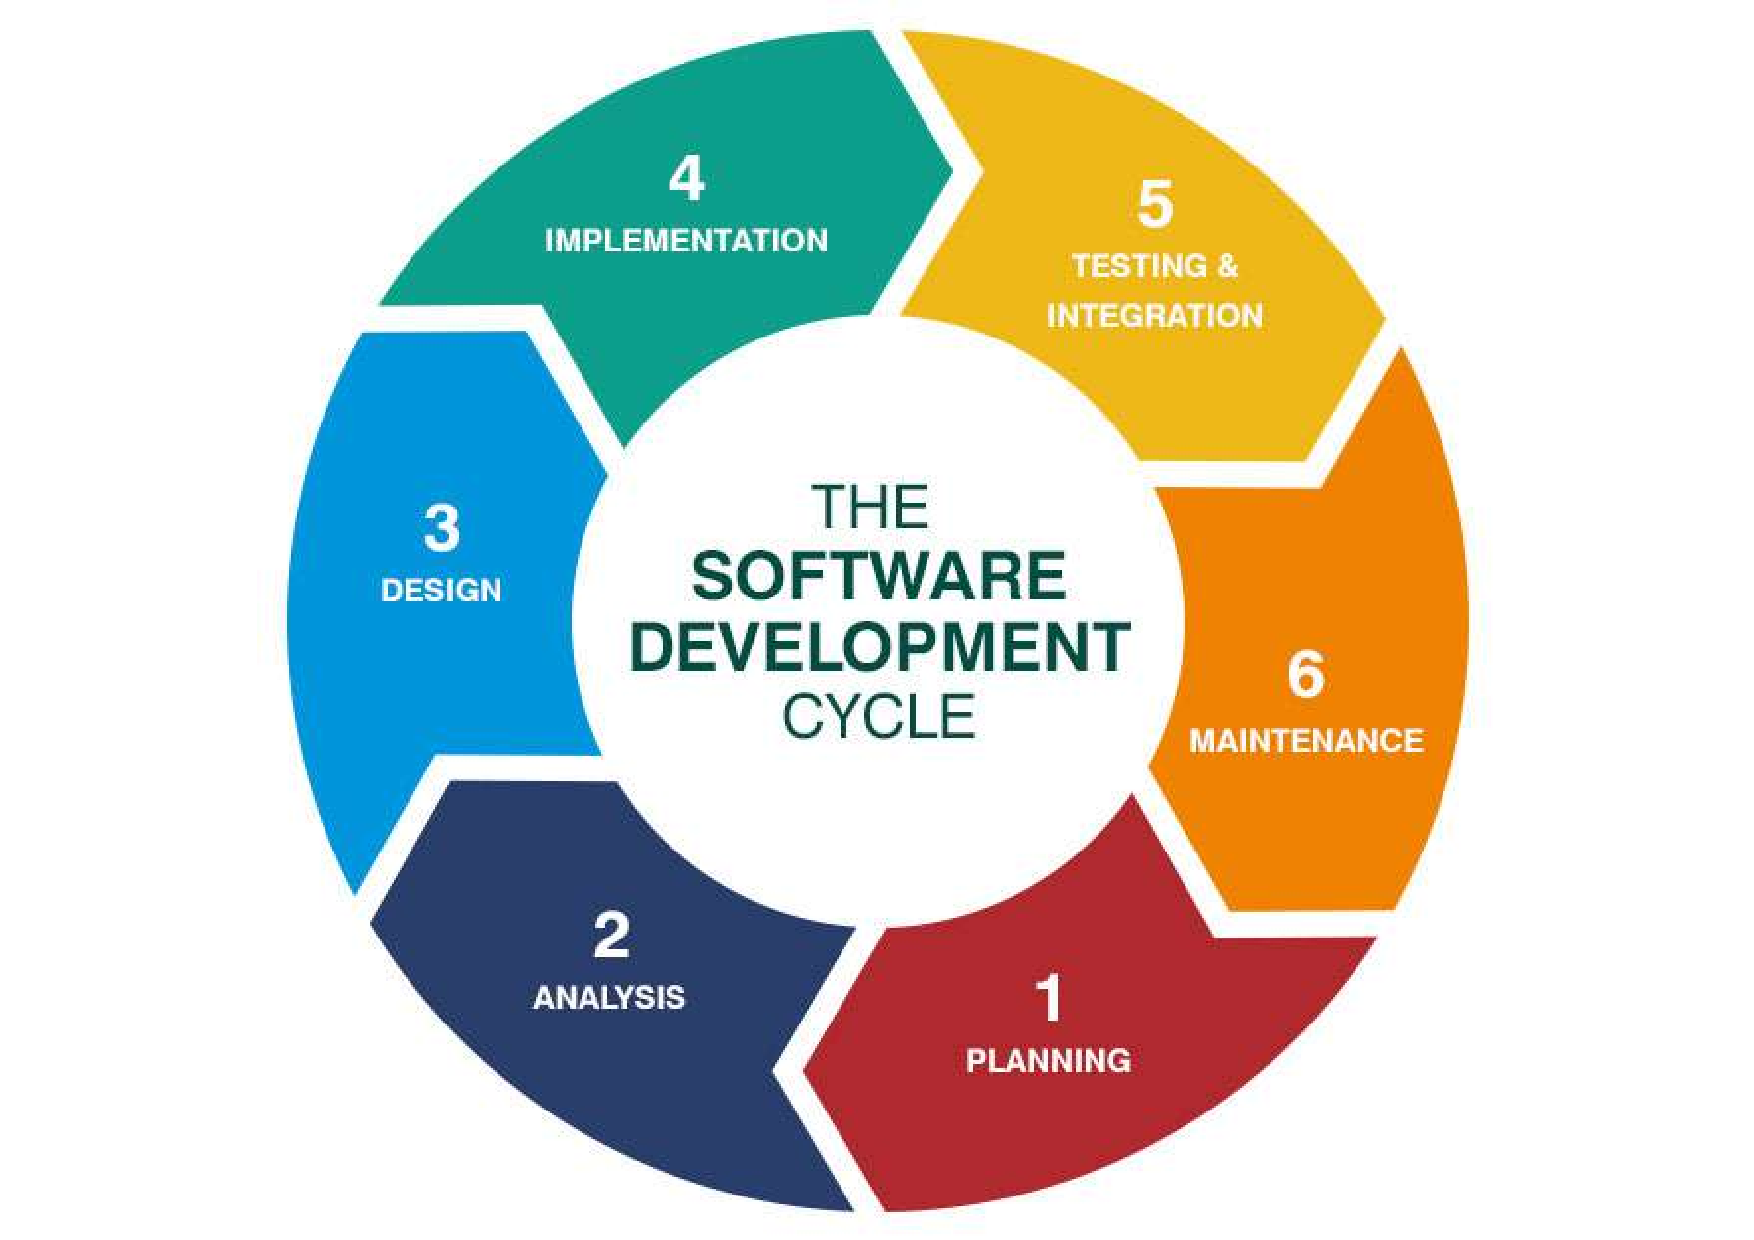
\includegraphics[width=0.6\linewidth]{figures/SDLC-stages.pdf}
    \caption{SDLC Stages (Replace with actual diagram)}
    \label{fig:sdlc}
\end{figure}

\subsection{Second Week:  Overall Activity / Topic Name (e.g. Practical Applications)}
\begin{itemize}
    \item \textbf{Hands-on Training:}
    \begin{itemize}
        \item Test case design and execution (See Table~\ref{tab:test-case-template}) \textcolor{red}{(You have to refer and describe every Table you mentioned in your report like above)}
        \item Bug reporting workflows
        \item Agile methodologies
    \end{itemize}
    \item \textbf{Tools Introduced:} Playwright, Postman
\end{itemize}

\begin{table}[H]
\centering
\caption{Sample Table}
\begin{tabular}{|l|p{8cm}|}
\hline
\textbf{Component} & \textbf{Description} \\ \hline
Test Case ID & Unique identifier \\ \hline
Test Scenario & Brief description \\ \hline
Test Steps & Detailed actions \\ \hline
Expected Result & Anticipated outcome \\ \hline
\end{tabular}
\label{tab:test-case-template}
\end{table}

\subsection{Third Week: Overall Activity / Topic Name (e.g. Automation)}
\begin{itemize}
    \item \textbf{Page Object Model:}
    \begin{itemize}
        \item Architecture design
        \item Implementation strategy
    \end{itemize}
    \item \textbf{Project Structure:}
    \begin{lstlisting}[style=tree]
project/
|-- pages/
|-- tests/
|-- utilities/
|-- .../
|-- .../
    \end{lstlisting}
\end{itemize}

\subsection{Fourth Week: Overall Activity / Topic Name (e.g. Advanced Concepts)}
\begin{itemize}
    \item \textbf{API Testing:} REST principles and practical implementation
    \item \textbf{Performance Testing:} JMeter fundamentals
    \item \textbf{Version Control:} Git/GitHub workflows
\end{itemize}

\section{Key Projects}
\textcolor{red}{You must include workflow diagrams, ER diagrams, or sequence/class diagrams, or alternatively, add screenshots of the projects you worked on during your internship. If any screenshots contain sensitive information, ensure you have proper authorization before including them. Additionally, clearly mention your role and contributions to the project, any models used, the outcomes achieved, and the business perspective or impact of the project.}
\subsection{Project 1: Web Application Testing} 
    \begin{itemize}
        \item Scope and objectives
        \item ER and related diagrams
        \item Tools used
        \item Outcomes
    \end{itemize}
    
\subsection{Project 2: API Test Automation} 
    \begin{itemize}
        \item Test coverage
        \item ER and related diagrams
        \item Challenges faced
        \item Solutions implemented
    \end{itemize}

\subsection{Project 3: ...}

\textcolor{red}{You must include Entity-Relationship (ER) diagrams and related diagrams similar to IDP2. If company policies restrict the use of original diagrams, you should use replica diagrams instead.}

% \section{Automation Testing Example}
% Below is a complete Python test automation script using Playwright that students can include in their report:

% \newpage

% \begin{lstlisting}[language=Python, caption={Demo Python Script}, label=code:demo]

% import pandas as pd

% def drop_row(csv_filename):
%     """Read a CSV file and dropped the first row"""
%     df = pd.read_csv(csv_filename)
%     return df.drop(0)

% df = drop_row("demo.csv")
% \end{lstlisting}

% Key Features Demonstrated:
% \begin{itemize}
%     \item Complete working test script
%     \item Browser automation with Playwright
%     \item Common test actions (navigation, assertions)
%     \item Proper error handling
%     \item Page object pattern basics
% \end{itemize}

% \textcolor{red}{This below section is optional}

\section{Other Responsibilities}

\textcolor{red}{(e.g. Team Management, Proposal Writing)}

\section{Key Performance Indicator}
\textcolor{red}{If you achieved any KPIs during your internship, be sure to include them with sufficient and relevant evidence.}

\section{Internship Summary}

\textcolor{red}{Mention bit details about your summary and learning, not necessarily exact to the below given format}

\par The industrial internship was a mandatory component of the undergraduate B.Sc. in Computer Science and Engineering program. It aimed to provide practical exposure and a real-world working environment to enhance academic learning with hands-on experience. The training focused on the application of theoretical knowledge to software development, debugging, collaboration, and use of modern tools in a professional setting.

\par The internship was conducted in a hybrid mode, combining remote project-based tasks with periodic in-person meetings for review and feedback. A variety of learning methodologies were adopted, including self-paced assignments, team collaboration, live mentoring sessions, and peer code reviews. The experience helped in developing technical competency, improving communication skills, and strengthening ethical awareness.

\textcolor{red}{Clearly mention the exact table rows along with your specific accomplishments and details.}

\par The key summary of the internship is presented in Table~\ref{tab:internship-summary}.

\begin{table}[H]
\centering
\caption{Internship Summary}
\label{tab:internship-summary}
\renewcommand{\arraystretch}{1.4}
\begin{tabularx}{\textwidth}{|>{\centering\arraybackslash}p{5cm}|>{\arraybackslash}X|}
\hline
\textbf{Parameter} & \textbf{Details} \\
\hline
\textbf{Organization Name} & [Insert Company/Organization Name] \\
\hline
\textbf{Internship Period} & [Insert Start Date] to [Insert End Date] \\
\hline
\textbf{Total Duration} & [e.g., 8 weeks (56 days)] \\
\hline
\textbf{Total Working Hours} & [e.g., 320 hours (approx.)] \\
\hline
\textbf{Mode of Internship} & Hybrid (Remote + Onsite) \\
\hline
\textbf{Nature of Work} & Software Development, Testing, Debugging, Documentation \\
\hline
\textbf{Tools and Technologies Used} & Git, Postman, JMeter, Firebase, Docker, SQL, JavaScript \\
\hline
\textbf{Learning Methodology} & Self-paced tasks, Live mentoring, Code reviews, Weekly stand-up meetings \\
\hline
\textbf{Reporting Mechanism} & Weekly progress reports and final project presentation \\
\hline
\textbf{Mentor/ Supervisor} & [Insert Mentor’s Name and Designation] \\
\hline
\end{tabularx}
\end{table}


\textcolor{red}{Mention a concluding summary of your learning in 3-4 lines, not necessarily exact to the below given format}

\par Overall, the internship provided a comprehensive platform to integrate academic concepts with practical industrial processes. It contributed significantly to the development of professional behavior, time management, technical proficiency, and alignment with Sustainable Development Goals (SDGs).

% \section{Conclusion}
% \begin{itemize}
%     \item Summary of key experiences
%     \item How training aligned with academic knowledge
%     \item Future application of learned skills
% \end{itemize}